% !TeX spellcheck = en_GB
\begin{figure}[h!]
	\centering
	%%%%%% 20/12
	\begin{subfigure}[b]{0.49\textwidth}
		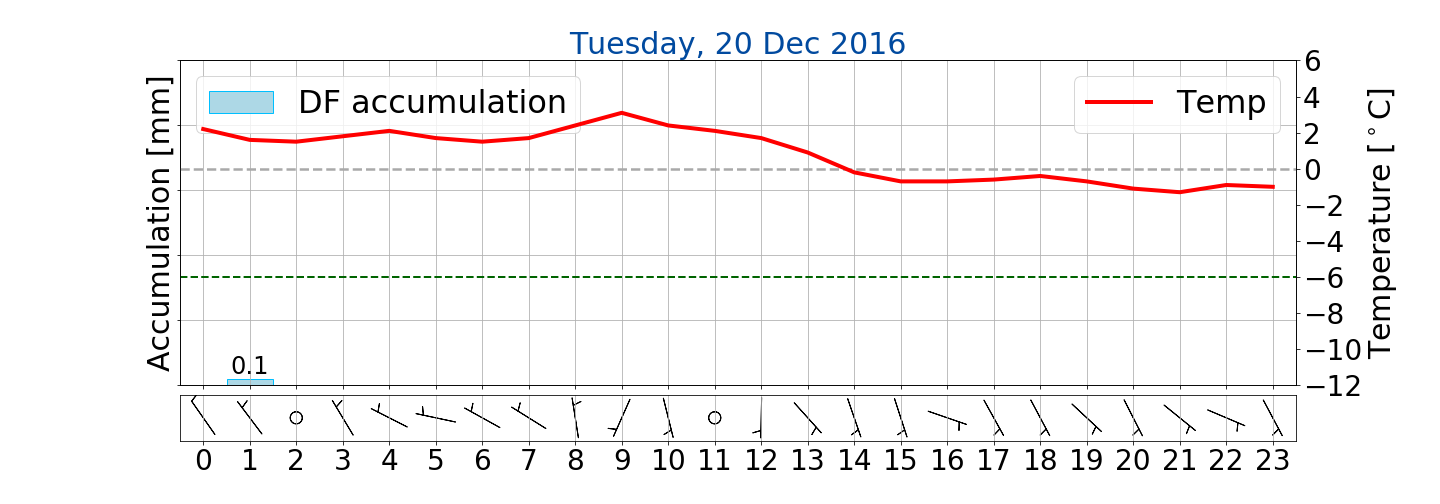
\includegraphics[trim={4.9cm 1.cm 1.5cm 1cm},clip,
		width=\textwidth]{./fig_weathermast/T_P_U_20161220}
		\caption{}\label{fig:TPU20}
	\end{subfigure}
	\hfill
	%%%%%% 21/12
	\begin{subfigure}[b]{0.49\textwidth}
		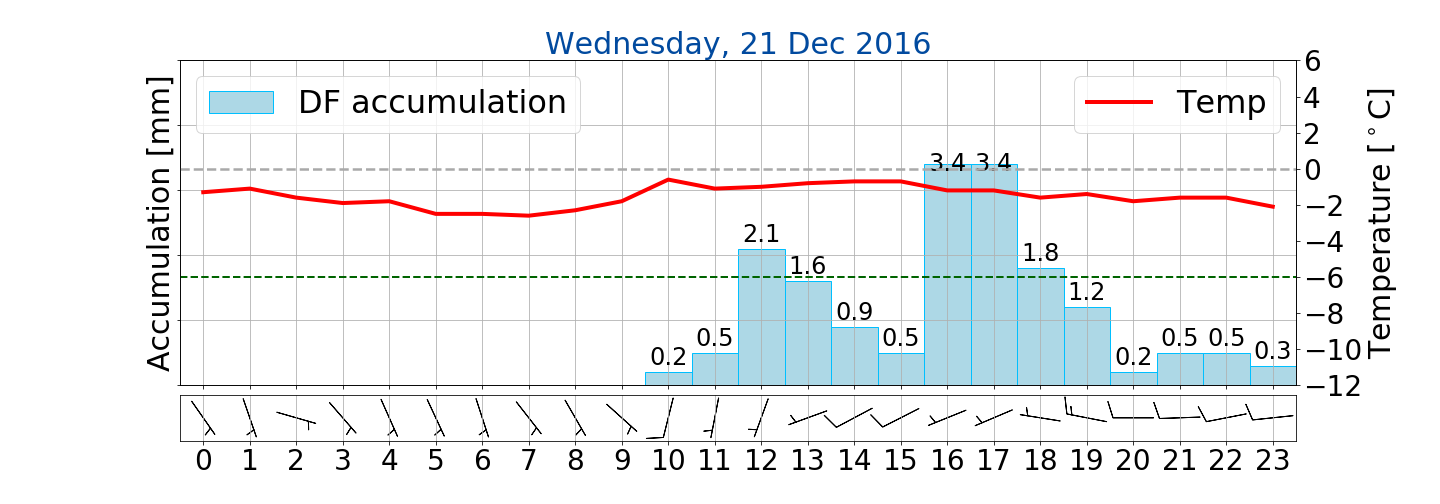
\includegraphics[trim={4.9cm 1.cm 1.5cm 1cm},clip,
		width=\textwidth]{./fig_weathermast/T_P_U_20161221}
		\caption{}\label{fig:TPU21}
	\end{subfigure}
% \end{figure}
% \begin{figure}\ContinuedFloat
	\centering
	%%%%%% 22/12
	\begin{subfigure}[b]{0.49\textwidth}
		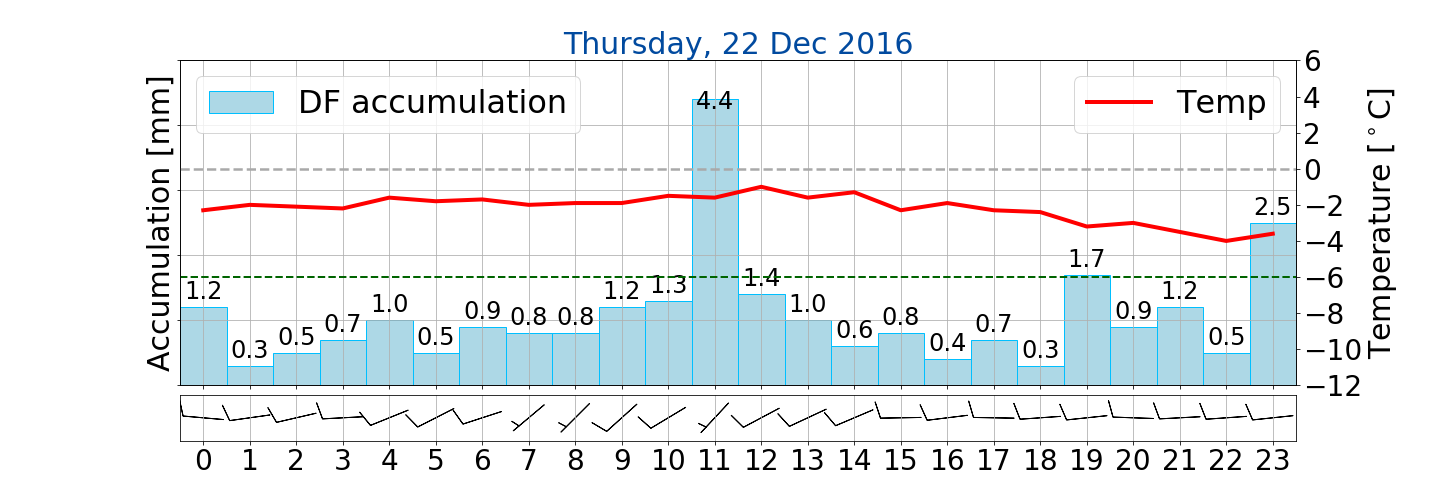
\includegraphics[trim={4.9cm 1.cm 1.5cm 1cm},clip,
		width=\textwidth]{./fig_weathermast/T_P_U_20161222}
		\caption{}\label{fig:TPU22}
	\end{subfigure}
	\hfill
	%%%%%% 23/12
	\begin{subfigure}[b]{0.49\textwidth}
		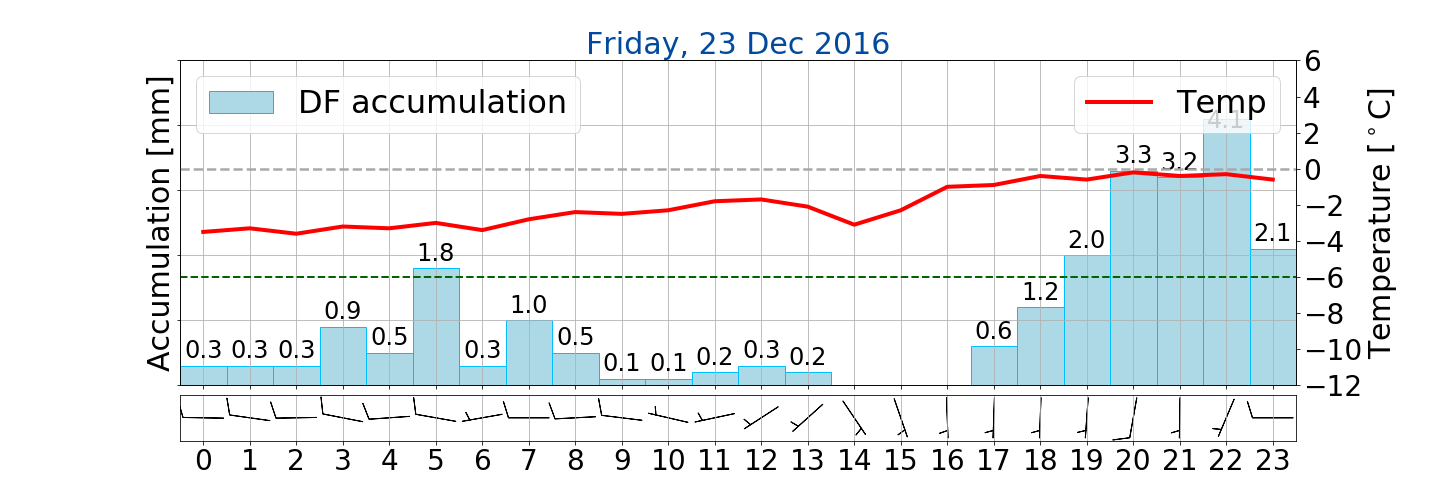
\includegraphics[trim={4.9cm 1.cm 1.5cm 1cm},clip,
		width=\textwidth]{./fig_weathermast/T_P_U_20161223}
		\caption{}\label{fig:TPU23}
	\end{subfigure}
	%\end{figure}
	%\begin{figure}[h]\ContinuedFloat
	%%%%%% 24/12
	\begin{subfigure}[b]{0.49\textwidth}
		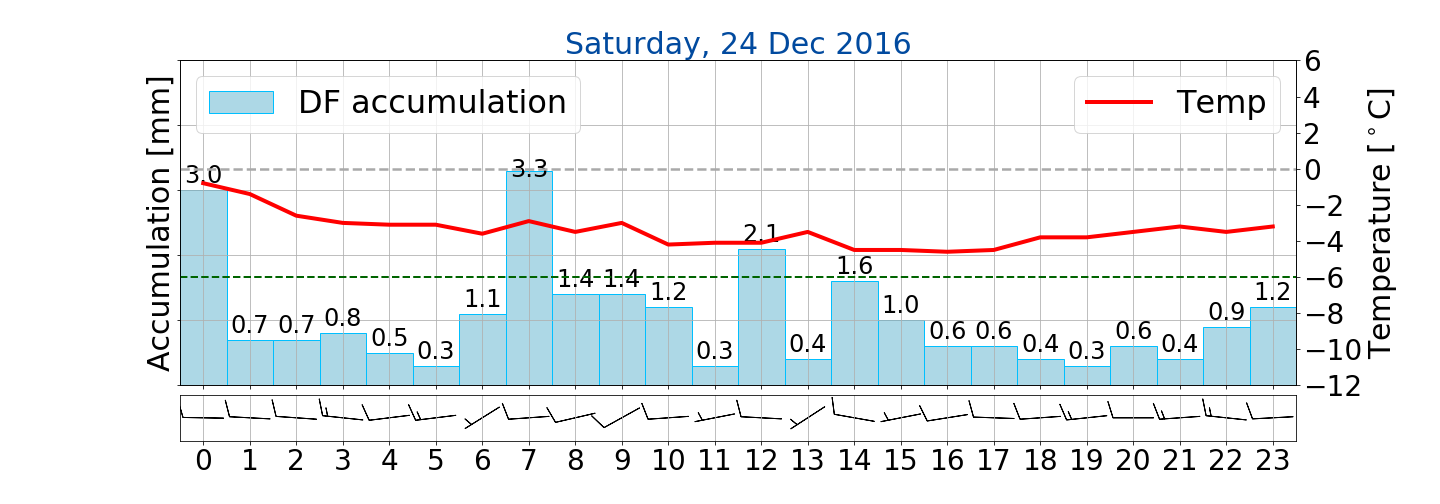
\includegraphics[trim={4.9cm 1.cm 1.5cm 1cm},clip,
		width=\textwidth]{./fig_weathermast/T_P_U_20161224}
		\caption{}\label{fig:TPU24}
	\end{subfigure}
	\hfill
	%%%%%% 25/12
	\begin{subfigure}[b]{0.49\textwidth}
		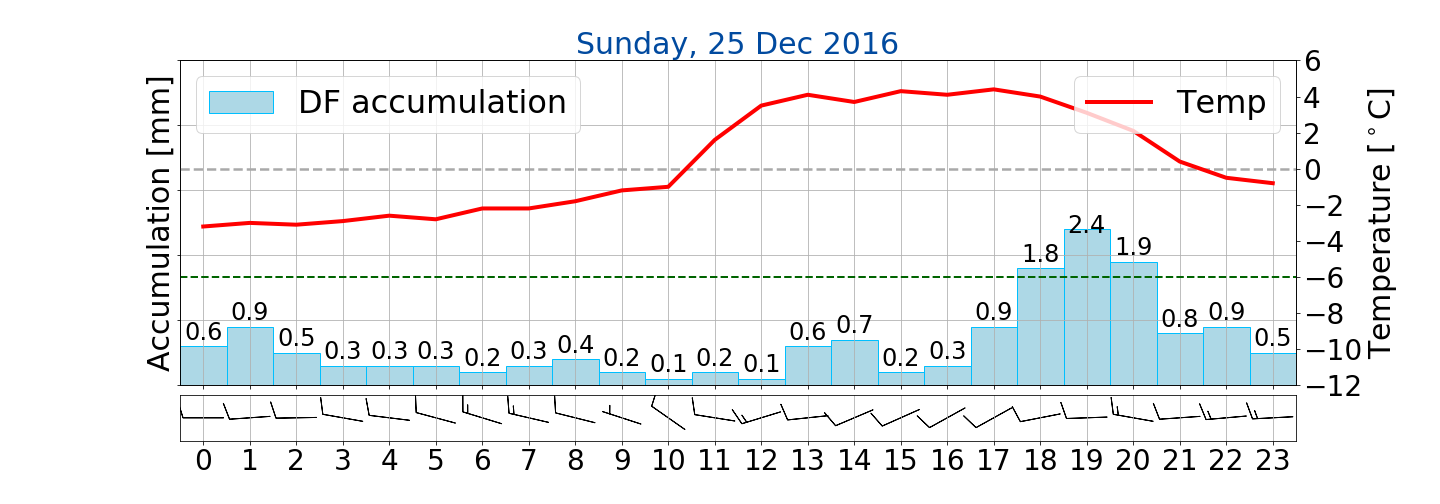
\includegraphics[trim={4.9cm 1.cm 1.5cm 1cm},clip,
		width=\textwidth]{./fig_weathermast/T_P_U_20161225}
		\caption{}\label{fig:TPU25}
	\end{subfigure}
	%%%%%% 26/12
	\begin{subfigure}[b]{0.49\textwidth}
		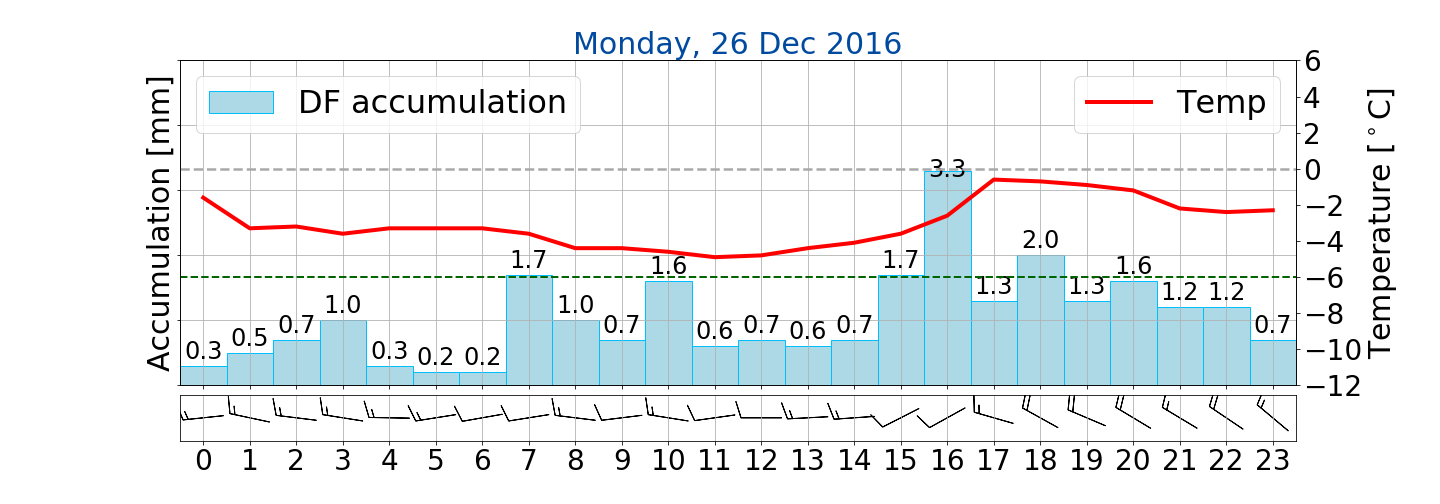
\includegraphics[trim={4.9cm 1.cm 1.5cm 1cm},clip,
		width=\textwidth]{./fig_weathermast/T_P_U_20161226}
		\caption{}\label{fig:TPU26}
	\end{subfigure}
	\hfill
	%%%%%% 27/12
	\begin{subfigure}[b]{0.49\textwidth}
		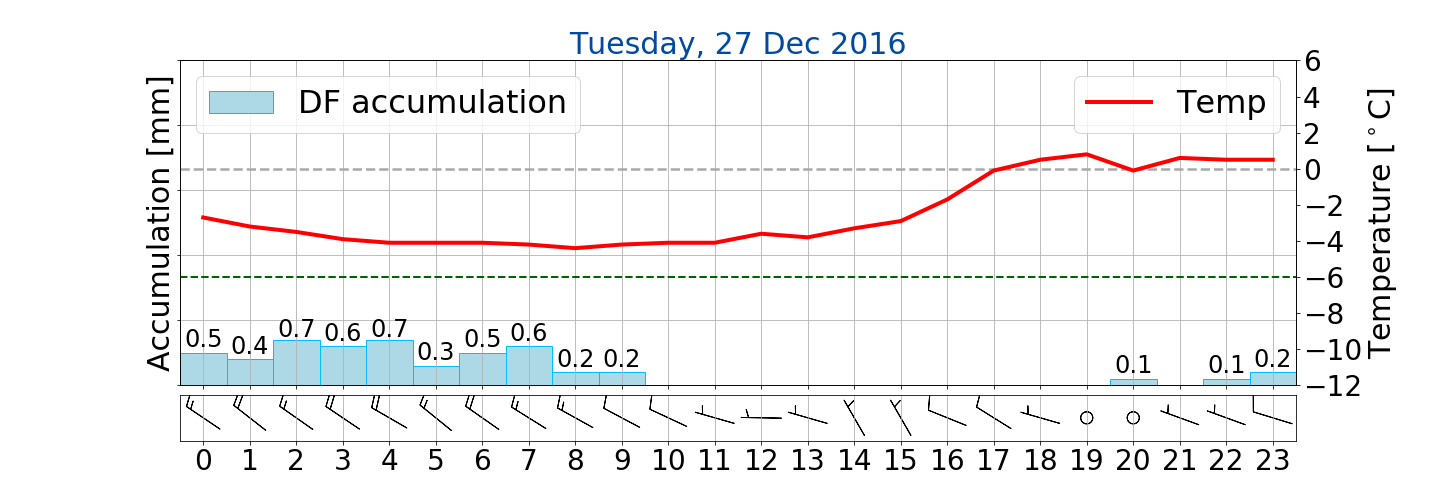
\includegraphics[trim={4.9cm 1.cm 1.5cm 1cm},clip,
		width=\textwidth]{./fig_weathermast/T_P_U_20161227}
		\caption{}\label{fig:TPU27}
	\end{subfigure}
	\caption{Observation from the weather mast at Haukeliseter during \SIrange{20}{27}{\dec}. \SI{60}{\minute} total accumulation [\SI{}{\mm}] in light blue as bar, temperature (red, [\SI{}{\celsius}]), and wind as barbs [\SI{}{\mPs}]. Gray dashed line indicates the freezing temperature and the green dashed line the 30-year climate mean temperature at \SI{-6}{\celsius}. Hourly processed data taken from \cite{eklima_norwegian_2016}.} \label{fig:TPU}
\end{figure}